\begin{center}
\begin{tikzpicture}[lablum/.style={name=img-#1},
marr/.style={line width=1mm,-latex}]
    \node[lablum=1] at (-1,0) {
    \tikzset{every picture/.style={line width=0.75pt}} %set default line width to 0.75pt        

\begin{tikzpicture}[x=0.75pt,y=0.75pt,yscale=-1,xscale=1, scale=0.5]
%uncomment if require: \path (0,300); %set diagram left start at 0, and has height of 300

%Curve Lines [id:da9540499645467757] 
\draw[very thick]    (200,80) .. controls (200.37,157.95) and (199.76,149.72) .. (199.86,159.97) .. controls (199.95,170.23) and (199.66,200.48) .. (239.95,200.48) .. controls (280.24,200.48) and (280.45,169.98) .. (280.43,160.26) .. controls (280.41,150.54) and (280,142.67) .. (280,80) ;
%Shape: Right Angle [id:dp9754098500167554] 
\draw[very thick]   (280.43,160.26) -- (319.53,160.26) -- (319.53,199.83) ;
%Shape: Circle [id:dp8187173182576306] 
\draw  [fill={rgb, 255:red, 0; green, 0; blue, 0 }  ,fill opacity=1 ] (316.96,160) .. controls (316.96,158.83) and (318.11,157.68) .. (319.53,157.68) .. controls (320.96,157.68) and (322.11,158.83) .. (322.11,160.26) .. controls (322.11,161.68) and (320.96,162.83) .. (319.53,162.83) .. controls (318.11,162.83) and (316.96,161.68) .. (316.96,160.26) -- cycle ;

\end{tikzpicture}
    } ;
    
    \node[lablum=2] at (2,0) {
    \tikzset{every picture/.style={line width=0.75pt}} %set default line width to 0.75pt        

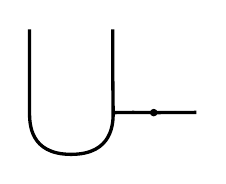
\begin{tikzpicture}[x=0.75pt,y=0.75pt,yscale=-1,xscale=1, scale=0.5]
%uncomment if require: \path (0,300); %set diagram left start at 0, and has height of 300

%Curve Lines [id:da8247822310570438] 
\draw[very thick]    (360,80) .. controls (360,157.95) and (359.92,149.72) .. (360.01,159.97) .. controls (360.1,170.23) and (359.82,200.48) .. (400.1,200.48) .. controls (440.39,200.48) and (440.6,169.98) .. (440.58,160.26) .. controls (440.56,150.54) and (440.15,142.67) .. (440.15,80) ;
%Shape: Circle [id:dp2701492263080221] 
\draw  [fill={rgb, 255:red, 0; green, 0; blue, 0 }  ,fill opacity=1 ] (477.11,160.26) .. controls (477.11,158.83) and (478.26,157.68) .. (479.69,157.68) .. controls (481.11,157.68) and (482.26,158.83) .. (482.26,160.26) .. controls (482.26,161.68) and (481.11,162.83) .. (479.69,162.83) .. controls (478.26,162.83) and (477.11,161.68) .. (477.11,160.26) -- cycle ;
%Straight Lines [id:da22484458939328644] 
\draw[very thick]    (440.58,160.26) -- (459.88,160.04) -- (479.69,160.26) -- (520.68,160.04) ;

\end{tikzpicture}
    } ;
    \node[lablum=3] at (5,0) {
   

\tikzset{every picture/.style={line width=0.75pt}} %set default line width to 0.75pt        

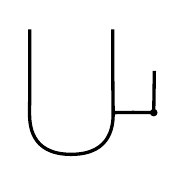
\begin{tikzpicture}[x=0.75pt,y=0.75pt,yscale=-1,xscale=1, scale=0.5]
%uncomment if require: \path (0,300); %set diagram left start at 0, and has height of 300

%Curve Lines [id:da8247822310570438] 
\draw[very thick]    (360.15,80) .. controls (360.52,157.95) and (359.92,149.72) .. (360.01,159.97) .. controls (360.1,170.23) and (359.82,200.48) .. (400.1,200.48) .. controls (440.39,200.48) and (440.6,169.98) .. (440.58,160.26) .. controls (440.56,150.54) and (440.15,142.67) .. (440.15,80) ;
%Shape: Circle [id:dp2701492263080221] 
\draw  [fill={rgb, 255:red, 0; green, 0; blue, 0 }  ,fill opacity=1 ] (477.11,160.26) .. controls (477.11,158.83) and (478.26,157.68) .. (479.69,157.68) .. controls (481.11,157.68) and (482.26,158.83) .. (482.26,160.26) .. controls (482.26,161.68) and (481.11,162.83) .. (479.69,162.83) .. controls (478.26,162.83) and (477.11,161.68) .. (477.11,160.26) -- cycle ;
%Straight Lines [id:da22484458939328644] 
\draw[very thick]    (440.58,160.26) -- (459.88,160.04) -- (479.69,160.26) -- (480.28,120.04) ;




\end{tikzpicture}

    } ;
    \node[lablum=4] at (8,0) {
   

\tikzset{every picture/.style={line width=0.75pt}} %set default line width to 0.75pt        

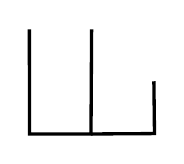
\begin{tikzpicture}[x=0.75pt,y=0.75pt,yscale=-1,xscale=1, scale=0.5]
%uncomment if require: \path (0,300); %set diagram left start at 0, and has height of 300

%Straight Lines [id:da08236342906025662] 
\draw[very thick]    (300,60) -- (300.2,160.84) -- (359.4,160.84) -- (360,60.03) ;
%Straight Lines [id:da480343613921552] 
\draw[very thick]    (359.4,160.84) -- (420.6,160.44) -- (420,110.03) ;


\end{tikzpicture}


    } ;
    \node[lablum=5] at (11,0) {
   

\tikzset{every picture/.style={line width=0.75pt}} %set default line width to 0.75pt        

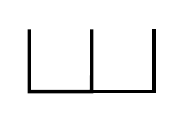
\begin{tikzpicture}[x=0.75pt,y=0.75pt,yscale=-1,xscale=1, scale=0.5]
%uncomment if require: \path (0,300); %set diagram left start at 0, and has height of 300

%Straight Lines [id:da08236342906025662] 
\draw[very thick]  (300,100) -- (300,160) -- (360,160) -- (360.2,100);
%Straight Lines [id:da480343613921552] 
\draw[very thick]  (360,160) -- (420,160) -- (420,100);




\end{tikzpicture}


    } ;
    \draw[thick, ->] (img-1) -- (img-2);
    \draw[thick, ->] (img-2) -- (img-3);
    \draw[thick, ->] (img-3) -- (img-4);
    \draw[thick, ->] (img-4) -- (img-5);
\end{tikzpicture}
\end{center}